\chapter{Smartphone-based Quadrotor Prototype} \label{ch:prototype}
In this chapter, the quadrotor prototype is presented. All the components that are used to build the prototype are described with the purpose of detailing the function that each component fulfils within the quadrotor. Furthermore, the specific parameters of the built quadrotor are shown and the procedure carried out to find them experimentally is explained. This is of great importance for the design of the controllers that allow the flight of the built system.
\\\\
In Fig. \ref{fig:hardwareoverview}, a small overview of the hardware related to the electrical signals within the quadrotor is presented. This overview shows the interrelation between the main components detailed below.
\begin{figure}[h]
	\begin{center}
		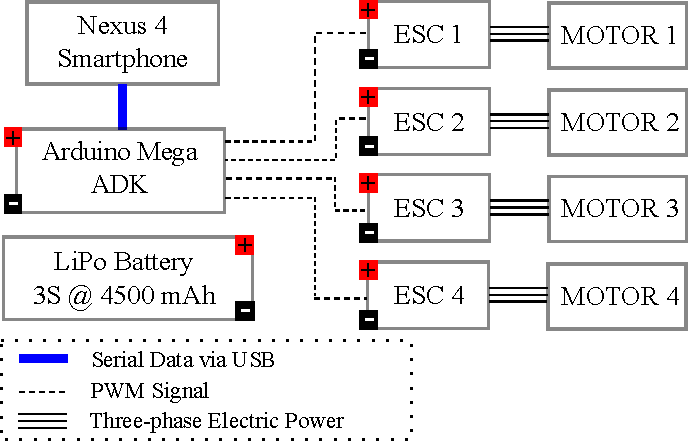
\includegraphics[width=13.0cm]{hardwareOverview}    
		\caption{Quadrotor prototype's hardware overview} 
		\label{fig:hardwareoverview}
	\end{center}
\end{figure}

\section{Quadrotor Components}
\label{sec:components}
The hardware used to build the quadrotor prototype is detailed in this section. The main goal of this research project is to control a quadrotor using just a smartphone on-board. This smartphone executes the state estimation algorithms and defines the controls signals that will command the actuators. The control signals are processed in the smartphone and then sent, through a gateway, to the Electronic Speed Controllers (ESCs) that will set the angular speed of the motors depending on the control signal they receive.
\subsection{Frame}
The quadrotor's frame is responsible for carrying all the other components needed in the system. Additionally, it must be able to support the weight of any possible payload that the quadrotor will carry. The multirotors frames are usually built using fiberglass or carbon fiber as main material, being the carbon fiber frames stiffer and lighter than equally built fiberglass frames.
\\\\
For this project, the requirement to build a quadrotor between $0.20$ and $0.30\ cm$ in radius was defined. This requirement is based on the fact that the quadrotor must carry a smartphone and possibly some mission-related payloads, which weight can be greater than $100\ g$. Taking that requirement and the literature review into account, in addition to the weight and stiffness advantages of the carbon fiber, a LJI 500-X4 carbon fiber frame was selected.
\begin{figure}[h]
\begin{center}
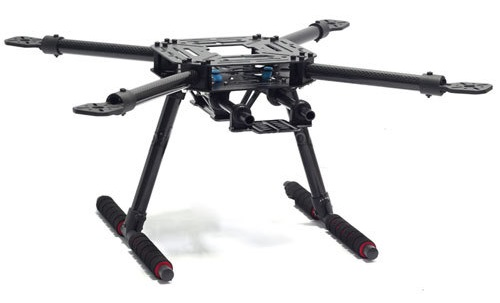
\includegraphics[width=8.6cm]{lji500x4.jpg}    
\caption[LJI 500-X4 carbon fiber frame]{LJI 500-X4 carbon fiber frame\protect\footnotemark} 
\label{fig:quadframe}
\end{center}
\end{figure}
\footnotetext{LJI 500-X4 frame image taken from \url{https://goo.gl/hHfHQR}}
\\
This frame (Fig. \ref{fig:quadframe}) has a weight of $431\ g$ and a radius $L$ of $0.244\ m$ measured between the frame center and each of the four rotor axis holes. Its landing gear has a height of $0.170\ m$, allowing the payload to be placed in the lower part of the quadrotor.

\subsection{Smartphone}
In this project, the smartphone takes the place of the quadrotor's flight controller. The basic instrumentation needed for a flight controller includes a triaxial accelerometer, a triaxial gyroscope, a triaxial magnetometer, a barometer and a GNSS receiver that can process signals from the GPS and GLONASS satellites constellations. On the other side, the processor of a flight controller must be powerful enough to execute the control and estimation algorithms within the sample time of the control system.
\\\\
The LG Nexus 5X, shown in Fig. \ref{fig:nexus}, is a smartphone developed by Google and assembled by LG, released in 2015 with the Android 6.0.1 operating system. This phone has a Hexa-core Qualcomm MSM8992 Snapdragon 808 CPU that includes four Cortex-A53 and two Cortex-A57 cores with 1.4 GHz and 1.8 GHz clock rate respectively and an Adreno 418 GPU. Its features also include 2 GB of RAM memory, 32 GB of Flash memory, total mass of 136 g and a 12.3 MP camera.
\\
\begin{figure}[H]
\begin{center}

\includegraphics[width=5.5cm]{nexus5x.jpg}    
\caption[LG Nexus 5X, smartphone used as flight controller]{LG Nexus 5X, smartphone used as flight controller\protect\footnotemark} 
\label{fig:nexus}
\end{center}
 \end{figure}
 \footnotetext{LG Nexus 5X image taken from \url{https://goo.gl/RxyDJd}}
 \vspace{-0.5cm}
This smartphone features all the needed instrumentation for a flight controller, specified previously. The maximum sample rates of the instrumentation contained in the LG Nexus 5X are described in Table \ref{tb:samplerates}.
\begin{table}[h]
\small
\begin{center}
\caption{Sample Rates of the Sensors in the Smartphone}\label{tb:samplerates}
\begin{tabular}{c|c}\hline
\rule{0pt}{3ex} Sensor & Sample rate $[Hz]$ \\\hline\hline
\rule{0pt}{3ex}Triaxis accelerometer &  $400$ \\[0.7ex]
Triaxis gyroscope &  $200$ \\[0.7ex]
Triaxis magnetometer & $50$ \\[0.7ex]
Barometer &  $10$ \\[0.7ex] 
GNSS &  $1$  \\[0.7ex]\hline
\end{tabular}
\end{center}
\end{table}
\\\\
The LG Nexus 5X smartphone was selected in this project mainly due to its computational and instrumentation capabilities in addition to its communication interfaces (Bluetooth 4.0, Wireless LAN, USB Type-C and GSM). Its powerful CPU handling a GPU enables the possibility of developments using the camera for visual odometry, and controllers whose execution represents a high computational load, which exceeds the limits of a standard microcontroller such as the ATmega 2560.
\\\\
As the quadrotor's flight controller, the smartphone receives remote orders from the quadrotor's pilot using wireless communication, while executing the sensorial, estimation and control algorithms. After the control signals are calculated, they are sent to the actuators as a serial data frame using the USB interface between the smartphone and a gateway that converts the serial data into PWM signals.

\subsection{Motors and Electronic Speed Controllers}
The actuation system of the quadrotor is composed by R/C-type brushless motors, propellers and ESCs. The LJI 500-X4 frame manufacturer recommends using motors with a RPM constant of $810\ KV$, which means that these motors can rotate at a speed of $810\ RPM$ for each Volt applied to it. This kind of motors are used in medium to big sized multirotors due to its thrust efficiency and thrust capacity.
\\\\
Following this recommendation, the EMAX MT2216II motors were selected. These motors, shown in Fig. \ref{fig:emaxmotor}, are labelled by its manufacturer as $810\ KV$ motors with a maximum current consumption of $9.8\ A$ and a maximum thrust of $6.6\ N$, when using a $10$-inch propeller.
\begin{figure}[H]
\begin{subfigure}{.5\linewidth}
\centering
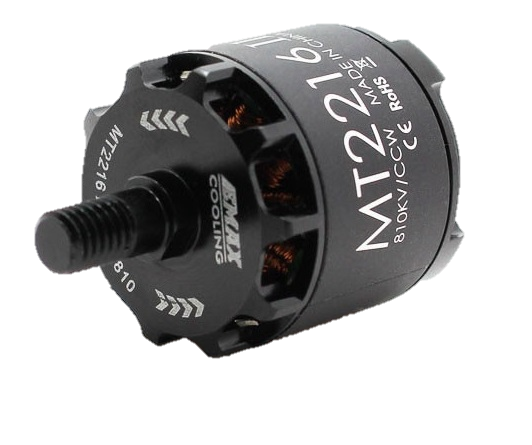
\includegraphics[width=5.6cm]{emax2216II2.png}    
\caption{EMAX MT2216II motor} 
\label{fig:emaxmotor}
\end{subfigure}
\begin{subfigure}{.5\linewidth}
\centering
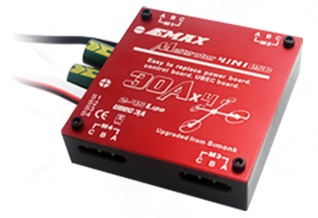
\includegraphics[width=7.0cm]{emax4in1.jpg}    
\caption{EMAX 4in1 ESC} 
\label{fig:emaxESC}
\end{subfigure}
\caption{Motors and ESC used in the Quadrotor\protect\footnotemark}
\label{fig:motorandesc}
\end{figure}
\footnotetext{Taken from \url{https://goo.gl/6qD6Qg} and \url{https://goo.gl/fDHiUp}}
The quadrotor's brushless motors are powered using a three-phase electric signal generated by the ESC. Each ESC sets one motor rotational velocity depending on a PWM signal input, and must be able to handle the maximum current consumption of the motor. Mainly due to the ease of handling and positioning within the frame, the EMAX 4in1 ESC was selected for this project (Fig. \ref{fig:emaxESC}). This 4in1 ESC contains four ESCs with a maximum current supply of $30\ A$ each. It also has a DC-DC converter that outputs an isolated $5\ V$ DC supply for any additional electronics. The power supply of the ESC is fully delivered by the quadrotor's battery.

\subsection{Smartphone-to-ESC Gateway}
As the smartphone can not generate any PWM signal and each ESC needs a PWM signal input to set the rotational velocity of a motor, a gateway between the smartphone and the ESCs must be used. In order to avoid interference in the electromagnetic spectrum and delays that could lead the control system to instability while using wireless communications, the smartphone wired serial bus (USB interface) is defined as the only channel of communication through which the control signals are sent to the gateway.
\\\\
The Arduino Mega ADK, is shown in Fig. \ref{fig:megaadk}, is a development board based on the Atmel 8-bit AVR RISC-based ATmega2560 microcontroller.  This board supports the Android Open Accesory (AOA) protocol, which allows external hardware to exchange data with Android devices.
\begin{figure}[H]
\begin{center}
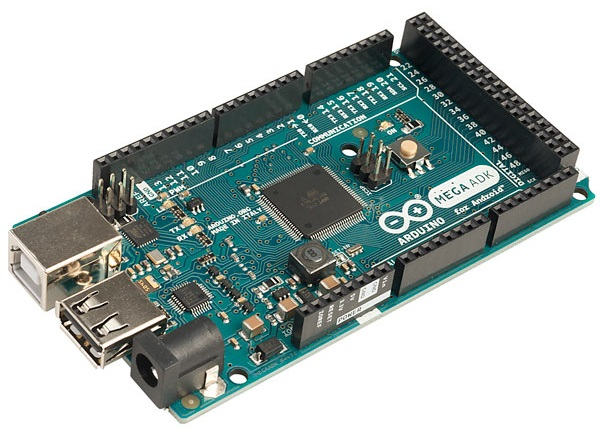
\includegraphics[width=7.6cm]{megaADK.jpg}    
\caption[Arduino Mega ADK]{Arduino Mega ADK\protect\footnotemark} 
\label{fig:megaadk}
\end{center}
 \end{figure}
 \footnotetext{Arduino Mega ADK image taken from \url{https://goo.gl/ejeQeX}}
\vspace{-0.5cm}
Although there are other boards that support the AOA protocol, as the IOIO board, the Arduino Mega ADK offers the possibility of executing tasks in the ATmega2560 microcontroller without any intervention of the Android device. This feature is very useful in case of future developments that include additional hardware to the smartphone-based quadrotor.
\\\\
The Arduino Mega ADK is selected as the smartphone-to-ESC gateway. The workflow of this board is set as follows: the microcontroller receives a serial data frame from the smartphone through the USB port, each of the four PWM signal widths is extracted from the data frame, the PWM signals are sent to the ESCs, finally the cycle starts again. This workflow is executed each $2\ ms$ and if the gateway does not receive any updated data frame from the smartphone, it keeps the last PWM signals set.

\subsection{Battery}
The quadrotor's battery must supply power to all the active components in the quadrotor. The maximum power consumption of these components, based on the nominal voltage value of a 3-cells lithium-ion polymer (LiPo) battery ($11.1\ V$), is shown below.\\
\begin{table}[h]
\small
\begin{center}
\caption{Maximum Power Consumption of the Quadrotor's Components}\label{tb:power}
\begin{tabular}{c|c|c|c}\hline
\rule{0pt}{3ex} Component & Voltage $[V]$ & Max. Current $[A]$ & Max. Power $[W]$ \\\hline\hline
\rule{0pt}{3ex}
Smartphone &  $5$ & $0.75$ & $3.75$ \\[0.4ex]
Arduino Mega ADK & $11.1$ & $0.75$ & $8.33$ \\[0.4ex] 
4 x ESCs &  $11.1$ & $1.38$ & $15.32$ \\[0.4ex]
4 x Motors & $11.1$ & $39.2$ & $435.12$ \\[0.4ex]\hline
\end{tabular}
\end{center}
\end{table}
\vspace{-0.5cm}
\\The maximum current consumption in the quadrotor reaches $42.08\ A$, so the battery must be able to deliver current amplitudes greater than that value. A Floureon 3-cells LiPo battery with a nominal capacity of $4500\ mAh$ and a nominal voltage of $11.1\ V$, was selected for this prototype and is shown in Fig. \ref{fig:battery}. This battery can deliver up to $30$ times its nominal current, this is $135\ A$, continuously.
\begin{figure}[H]
	\begin{center}
		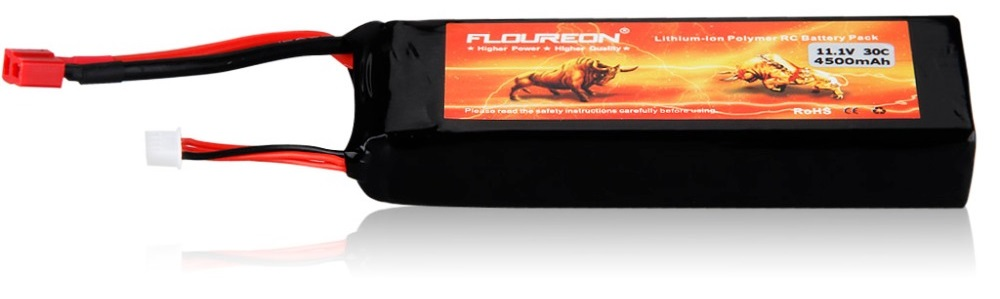
\includegraphics[width=9.0cm]{floureon.jpg}    
		\caption[LiPo battery that powers the Quadrotor]{LiPo battery that powers the Quadrotor\protect\footnotemark} 
		\label{fig:battery}
	\end{center}
\end{figure}
\footnotetext{Floureon 3S LiPo battery image taken from \url{https://goo.gl/anC9M2}}

\subsection{3D-printed Parts}
The smartphone, the Arduino Mega ADK and the 4in1 ESC need to be easily placed and protected when installed on the frame. For that reason, multiple support components and one case were designed and 3D-printed using polylactic acid (PLA) filament. These 3D-printed objects are detailed below.

\subsubsection{Smartphone Support}
In order to place the smartphone near the $CoG$ in the quadrotor and enable the possibility of capturing nadir photos or videos, the smartphone support is designed in such a way that it can be placed under the quadrotor's $CoG$ but above the landing gear of the frame. Additionally, the support includes a free area that allows to use the complete field of view of the camera without being obstructed by it. The smartphone support is shown in Fig. \ref{fig:phonesupport}.
\begin{figure}[h]
	\begin{center}
		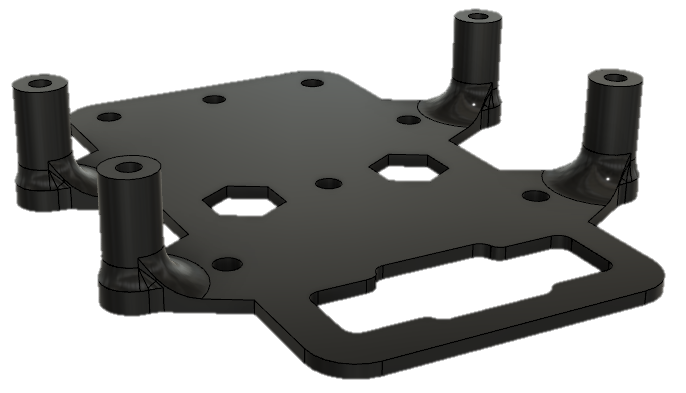
\includegraphics[width=8.6cm]{phonesupport2.png}    
		\caption{Smartphone support} 
		\label{fig:phonesupport}
	\end{center}
\end{figure}
\vspace{-0.5cm}
\subsubsection{Arduino Mega ADK and ESC supports}
The Arduino Mega ADK and the Emax 4in1 ESC are placed on the frame, above the quadrotor's $CoG$. Given the limited space available to locate these components on the top of the frame, their supports are designed to be placed one on top of the other, as shown in Fig. \ref{fig:megaandescsupports}.
\begin{figure}[h]
\begin{subfigure}{.5\linewidth}
\centering
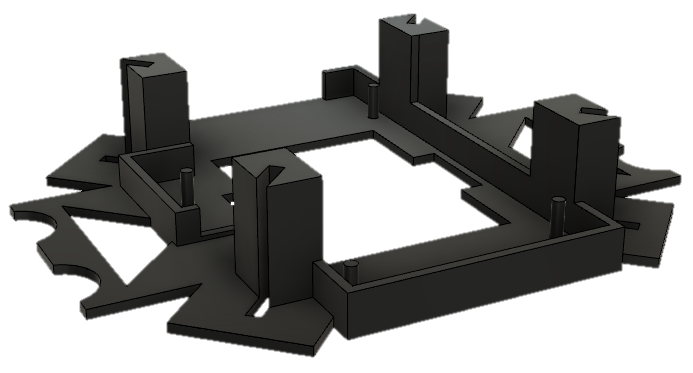
\includegraphics[width=7.0cm]{megasupport2.png}
\caption{Arduino Mega ADK support} 
\label{fig:megasupport}
\end{subfigure}%
\begin{subfigure}{.5\linewidth}
\centering
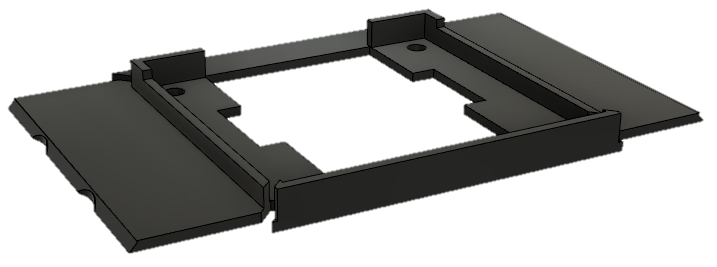
\includegraphics[width=7.0cm]{escsupport2.png}
\caption{ESCs support} 
\label{fig:escsupport}
\end{subfigure}\\[1ex]
\begin{subfigure}{\linewidth}
\centering
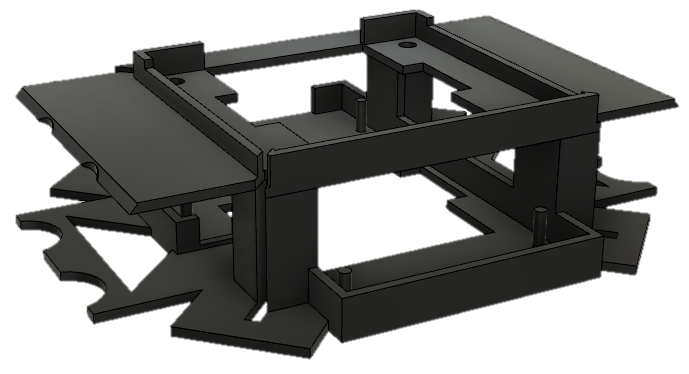
\includegraphics[width=7.0cm]{megaandescsupport2.png}
\caption{Arrangement of the Gateway and ESCs Support as a Whole} 
\label{fig:megaandescsupport}
\end{subfigure}
\caption{Arduino Mega ADK and EMAX 4in1 ESCs designed supports}
\label{fig:megaandescsupports}
\end{figure}

\subsubsection{Dome}
To protect the Arduino Mega ADK and the ESCs, a dome that covers and encloses them is designed. This dome, shown in Fig. \ref{fig:dome}, totally encloses the Mega ADK and ESCs supports restricting their movement and protecting them in case of a shock or hit.
\begin{figure}[H]
	\begin{center}
		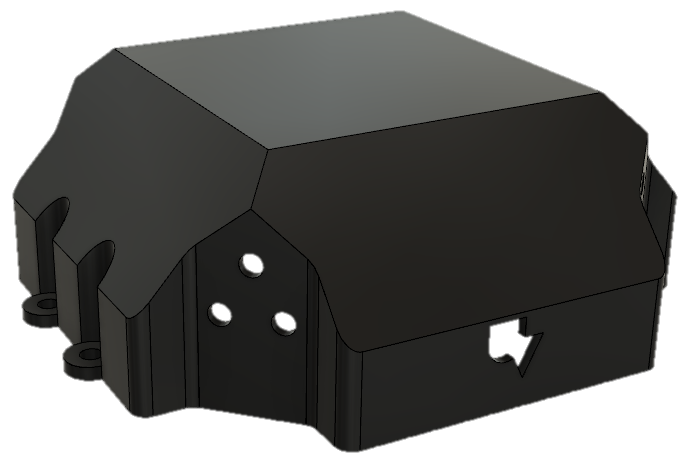
\includegraphics[width=8.6cm]{dome2.png}    
		\caption{3D Designed Dome} 
		\label{fig:dome}
	\end{center}
\end{figure}

\subsection{Assembled Smartphone-based Quadrotor}
The smartphone-based quadrotor prototype is assembled using all the components exposed in this section, and is shown in Fig. \ref{fig:completequad}.
\begin{figure}[H]
	\begin{center}
		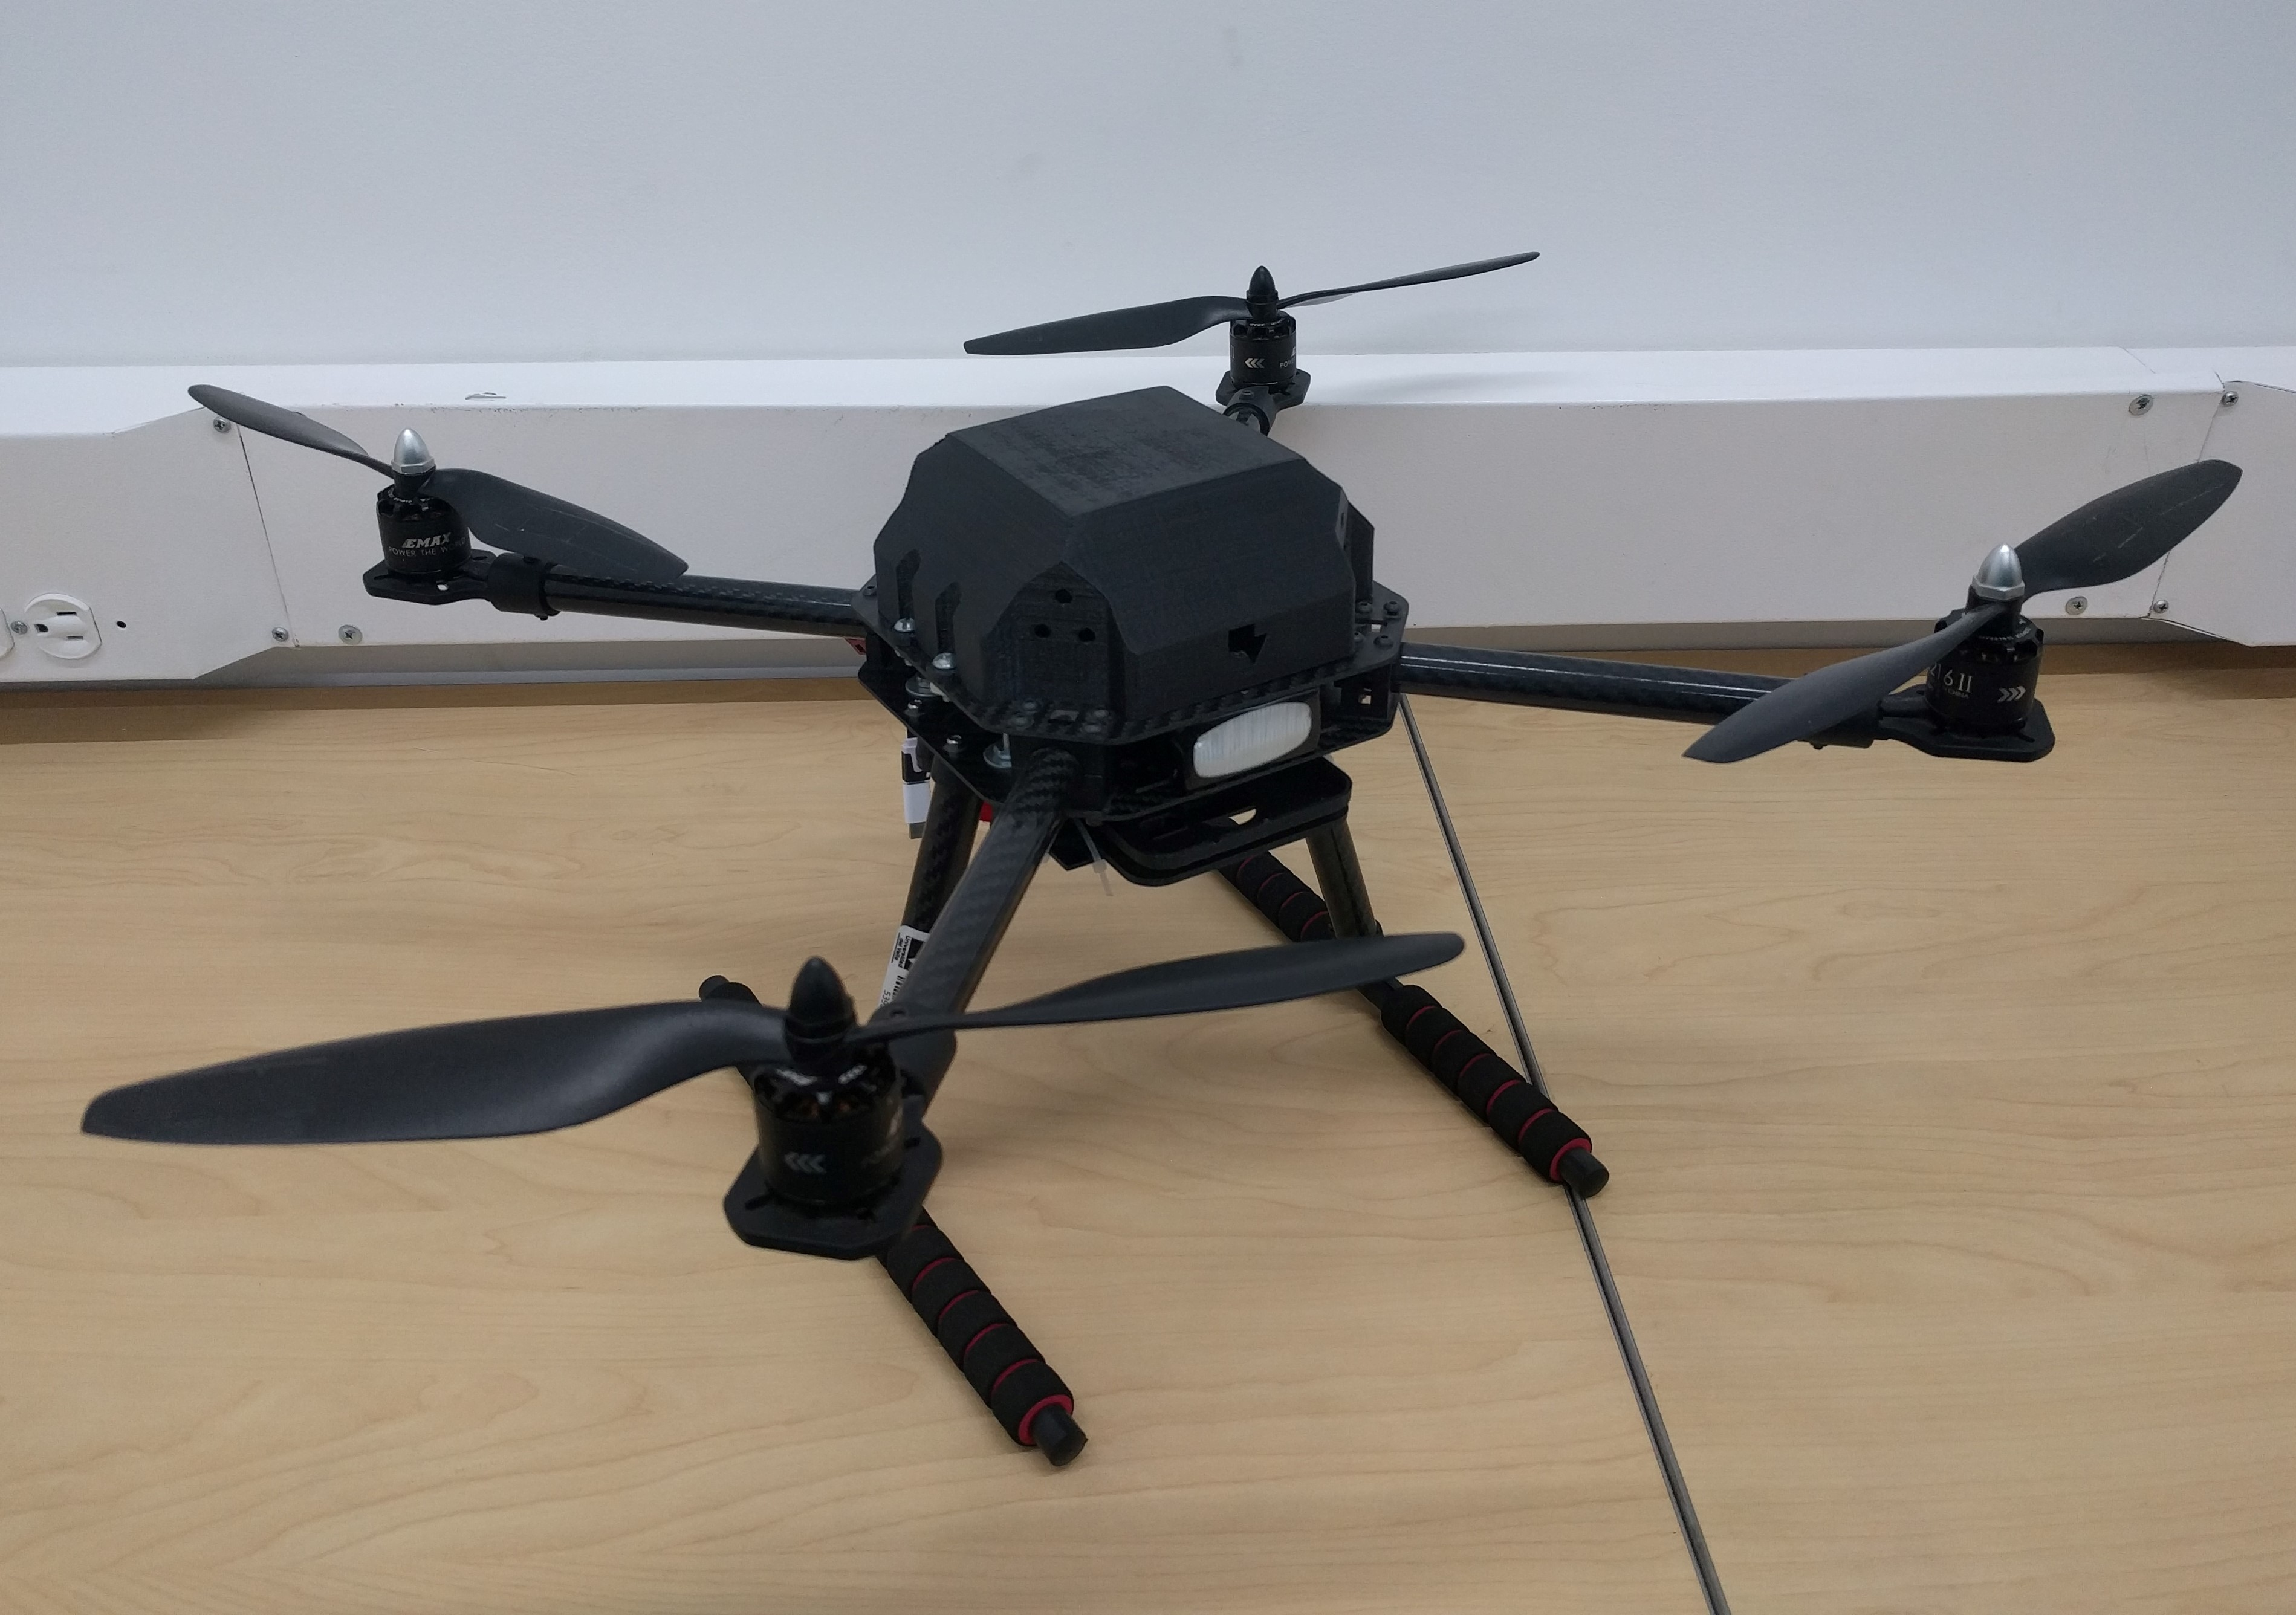
\includegraphics[width=14cm]{complete.jpg}    
		\caption{Assembled Smartphone-based Quadrotor Prototype} 
		\label{fig:completequad}
	\end{center}
\end{figure}

\section{Quadrotor Parameters} \label{sec:parameters}
In this section, the quadrotor parameters are detailed. These parameters define the specific dynamic model for the smartphone-based quadrotor prototype and the conversion of control signals to correctly set the motors thrust.
\subsection{Mass}
The mass of each quadrotor's component is measured using a kitchen scale that has an uncertainty of $\pm 1\ g$. The results are shown in Table \ref{tb:mass}.
\begin{table}[h]
\small
\begin{center}
\caption{Mass values of all the Quadrotor's components}\label{tb:mass}
\begin{tabular}{c|c}\hline
\rule{0pt}{3ex} Component & Mass $[kg]$ \\\hline\hline
\rule{0pt}{3ex}Smartphone &  $0.136$ \\[0.7ex]
Frame &  $0.431$ \\[0.7ex]
Battery & $0.351$ \\[0.7ex]
ESC &  $0.110$ \\[0.7ex] 
Arduino Mega ADK &  $0.330$ \\[0.7ex]
Motors (4) & $0.140$ \\[0.7ex]
Propellers (4) &  $0.380$ \\[0.7ex]
Smartphone support &  $0.105$ \\[0.7ex]
ADK support &  $0.590$  \\[0.7ex]
ESC support &  $0.350$  \\[0.7ex]
Dome &  $0.130$ \\[0.7ex]\hline
\rule{0pt}{3ex} Total & $1.568$
\end{tabular}
\end{center}
\end{table}
\\\\The total mass of the quadrotor $m$ is then calculated as the sum of the weight of each of the components in the quadrotor, being $m = 1.568\ kg$.
\subsection{Moments of Inertia}
As exposed by \cite{Lee2011}, in a quadrotor, the moment of inertia matrix $J$ is set as
\begin{equation}
J = \begin{bmatrix}
J_{xx} & -J_{xy} & -J_{xz} \\
-J_{yx} & J_{yy} & -J_{yz} \\
-J_{zx} & -J_{zy} & J_{zz}
\end{bmatrix}.
\end{equation}
Taking into account that the quadrotor's symmetry with respect to the $x$ and $y$ axes is assumed, the $J$ matrix can be approximated to
\begin{equation}
J  	\approx  \begin{bmatrix}
J_{xx} & 0 & 0 \\
0 & J_{yy} & 0 \\
0 & 0 & J_{zz}
\end{bmatrix}.
\end{equation}
The $J_{xx}$, $J_{yy}$ and $J_{zz}$ values can be obtained using multiple methods including: using a CAD model of the quadrotor and obtaining the inertia values from a 3D design software (\cite{Khodja2017}), approximating the shape of the quadrotor components to cylinders, cubes and other basic shapes to simplify the mathematical calculation of inertia (\cite{Tomas2011}), and developing the bifilar pendulum experiment on the quadrotor (\cite{Garcia2017}). For this project, it was decided to obtain the quadrotor parameters experimentally, so the bifiliar pendulum experiment was developed.
\\\\
In the bifilar pendulum experiment, an object is hung from two parallel ropes of length $r$ and separated by a distance $2l$, being allowed to rotate freely around a the axis that is parallel to the ropes. In Fig. \ref{fig:bifilar}, the geometry of the experiment to get  $J_{zz}$, is shown. For the $J_{xx}$ and $J_{yy}$ inertias experiment, it is necessary to place the quadrotor hanging in such a way that the $x$ and $y$ axes are pointing paraller to the ropes, respectively.
\begin{figure}[h]
	\begin{center}
		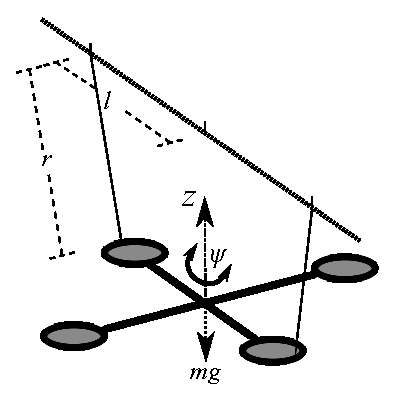
\includegraphics[width=6.0cm]{quadrotorInertia1}    
		\caption{Bifilar pendulum experiment geometry for inertia identification} 
		\label{fig:bifilar}
	\end{center}
\end{figure}
\\Once the quadrotor is hanging from the ropes, a small torque is applied manually to the quadrotor making it rotate about the vertical axis. The tension in the ropes makes the quadrotor swing, with a period of $T_{osc}$ [$s$], about the rotation axis.
\\\\
The moment of inertia is then calculated using the bifiliar equation
\begin{equation}
J.. = \dfrac{m|\vec{g}|T_{osc}^{2}l^{2}}{4\pi^{2}r}\ [kg\cdot m^{2}],
\end{equation}
where $m = 1.568\ kg$ is the quadrotor's total mass and $|\vec{g}| = 9.807\ m/s^{2}$ is the gravity acceleration magnitude (\cite{Mustapa2016}).
\\\\
In Fig. \ref{fig:inertiatest}, it is shown the excursion of the rotation angles, $\phi$, $\theta$ and $\psi$, about the $x$, $y$ and $z$ axes respectively, while performing the bifilar pendulum experiment separately.
\begin{figure}[H]
\begin{subfigure}{.5\linewidth}
\centering
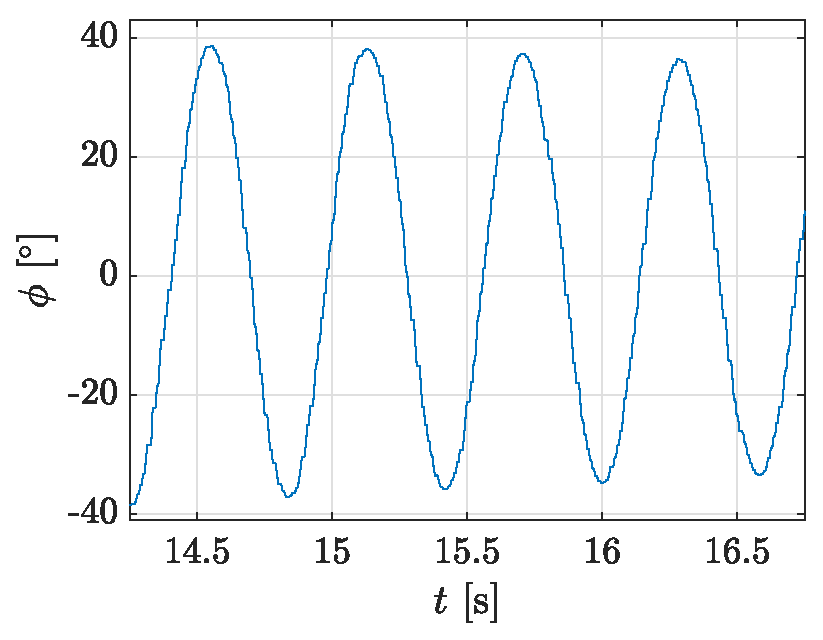
\includegraphics[width=7.0cm]{Ixx}
\caption{Rotation about $x$ axis, $J_{xx}$ experiment}
\label{fig:Jxx}
\end{subfigure}%
\begin{subfigure}{.5\linewidth}
\centering
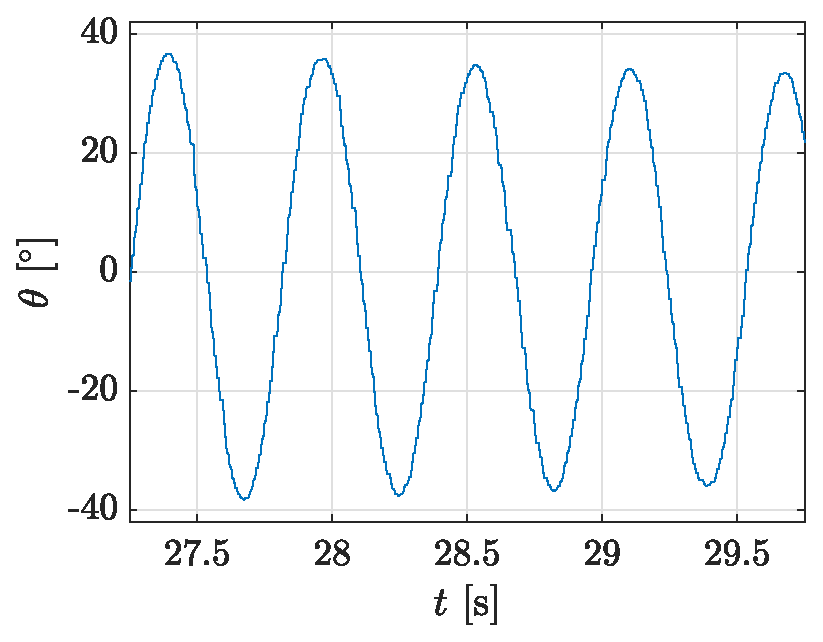
\includegraphics[width=7.0cm]{Iyy}
\caption{Rotation about $y$ axis, $J_{yy}$ experiment}
\label{fig:Jyy}
\end{subfigure}\\[1ex]
\begin{subfigure}{\linewidth}
\centering
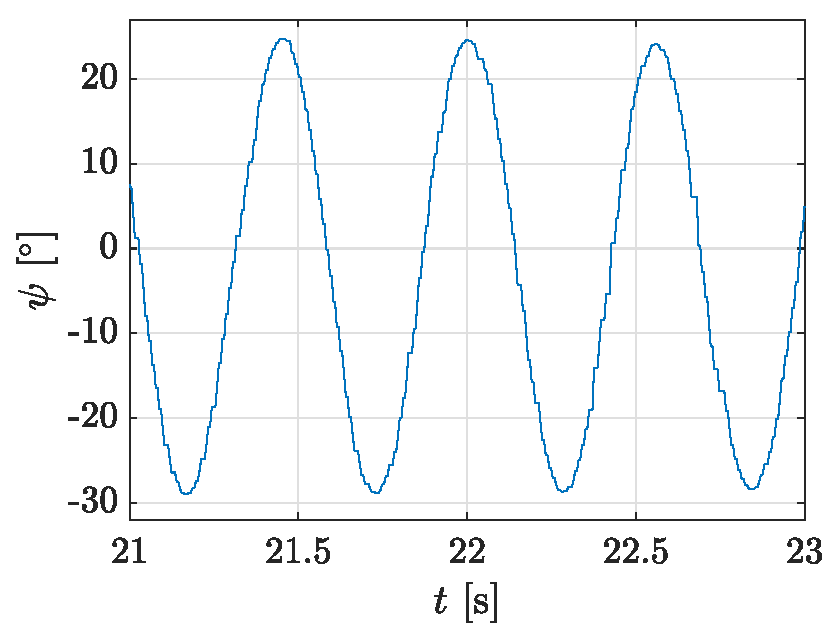
\includegraphics[width=7.0cm]{Izz}
\caption{Rotation about $z$ axis, $J_{zz}$ experiment}
\label{fig:Jzz}
\end{subfigure}
\caption{Rotation about $x$, $y$ and $z$ axes during the bifilar pendulum experiments}
\label{fig:inertiatest}
\end{figure}
The resulting data got after the execution of the experiment around the three components of the quadrotor body frame, are shown in Table \ref{tb:inertiaexperiment}.
\begin{table}[H]
\small
\begin{center}
\caption{Bifilar pendulum experiment results}\label{tb:inertiaexperiment}
\begin{tabular}{c|c|c|c|c}\hline
\rule{0pt}{3ex} Rotation Axis & $r$ [$m$] & $l$ [$m$] & $T_{osc}$ [$s$] & Inertia value [$kg\cdot m^{2}$] \\\hline\hline
\rule{0pt}{3ex} $x$ &  $1.18$ & $0.173$ & $1.168$ & $J_{xx} = 0.0135$ \\[0.7ex]
$y$ &  $1.10$ & $0.173$ & $1.080$ & $J_{yy} = 0.0124$ \\[0.7ex]
$z$ &  $1.025$ & $0.265$ & $1.122$ & $J_{zz} = 0.0336$ \\[0.7ex]\hline
\end{tabular}
\end{center}
\end{table}

\subsection{Motors Thrust}
As seen in Section \ref{sec:components}, the motors rotational velocity $\omega_{i}$ is set by the ESC, which receives a $PWM$ signal input. However, the inputs of the quadrotor ($u$, $\tau_\psi$, $\tau_\theta$, and $\tau_\phi$) depend on the thrust force $F_{M_{i}}$ applied by each quadrotor motor, as exposed in Section \ref{sec:inputsetting}.
\\\\
In order to correctly set the desired force $F_{M_{i}}$ in each motor during a flight, it is necessary to characterize the motor; and thus know how the force applied by the motor behaves with respect to the input $PWM$ signal. This characterization is carried out by means of a thrust test.
\\\\
In the thrust test, the motor and its corresponding propeller are fixed pointing up over a calibrated scale, as shown in Fig. \ref{fig:thrusttest}, while connected to the ESC, and then the \textit{PWM} signal is increased with steps of $10$, with $0$ being the minimum width of \textit{PWM} signal and $255$ the maximum, until reaching the maximum \textit{PWM} width. 
\begin{figure}[h]
	\begin{center}
		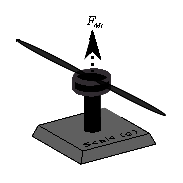
\includegraphics[width=7.0cm]{thrustTest}    
		\caption{Thrust test configuration} 
		\label{fig:thrusttest}
	\end{center}
\end{figure}
\\With each  \textit{PWM} signal width increment, a scale reading is made. Since the readings $m_{s}$ are obtained in units of mass ($kg$), the $F_{M_i}$ must be calculated as
\begin{equation}
F_{M_i} = m_{s}|\vec{g}|\ [N].
\end{equation}
This test was developed twice with each motor and its results are shown in Fig. \ref{fig:motor}.
\begin{figure}[H]
\begin{subfigure}{.5\linewidth}
\centering
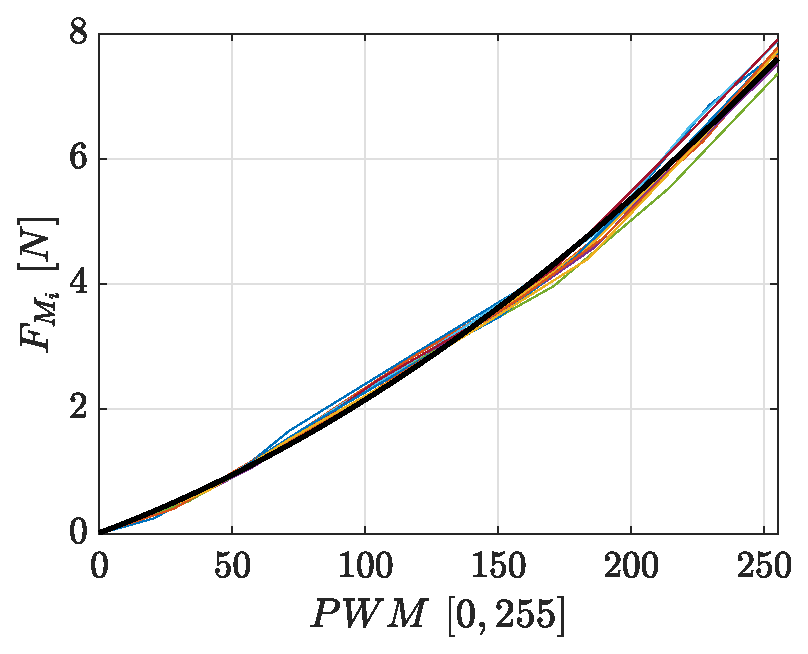
\includegraphics[width=7.0cm]{motorNvsPWM}
\caption{Motors characterization}
\label{fig:motor}
\end{subfigure}%
\begin{subfigure}{.5\linewidth}
\centering
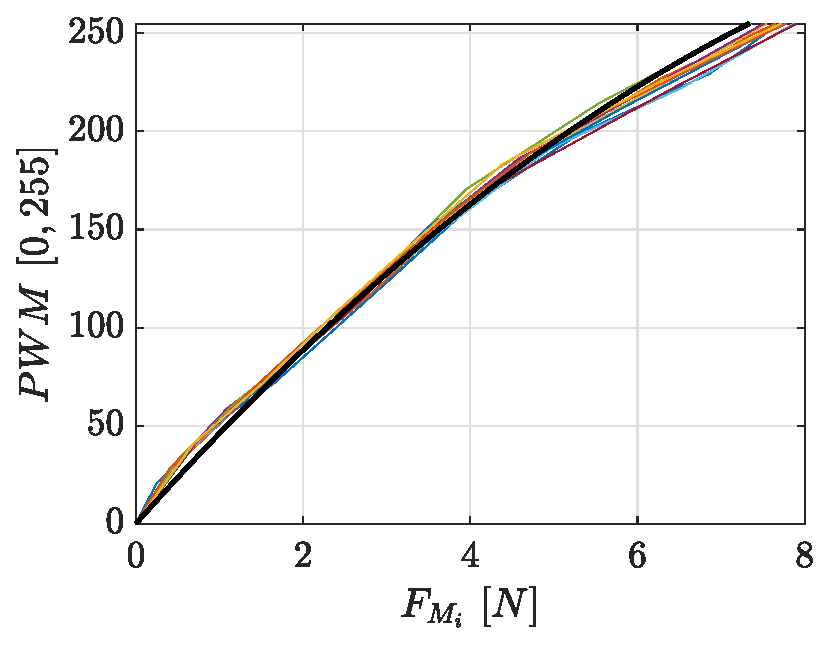
\includegraphics[width=7.0cm]{motorPWMvsN}
\caption{Inverse motors characterization}
\label{fig:inversemotor}
\end{subfigure}
\caption{Motors thrust test results}
\label{fig:test}
\end{figure}
In Fig. \ref{fig:inversemotor}, the inverse characterization is exposed. In this case, the \textit{PWM} signal is defined as the dependent variable, and $F_{M_i}$ as independent. This inverse characterization defines the \textit{PWM} width setting that is sent from the smartphone to the Arduino Mega ADK.
\\\\
The trend equations resulting from the thrust test are
\begin{equation}
\label{eqn:thrustvspwm}
F_{M_i} = (5.441\times10^{-5})(PWM)^{2} + 0.01586(PWM) + 0.014808,
\end{equation}
\begin{equation}
\label{eqn:pwmvsthrust}
PWM = -1.983F_{M_i}^{2} + 47.84F_{M_i} + 3.835,
\end{equation}
where $F_{M_i}$ is given in $N$, and \textit{PWM} is a value between $0$ and $255$.
\subsection{Motors Torque}
The quadrotor suffers the application of a torque $\tau_{M_{i}}$ around the $z$ axis when a motor $M_i$ rotates. This torque affects the $\psi$ angle indirectly by adding to the $\tau_\psi$ torque proportionally to the thrust force $F_{M_i}$, as
\begin{equation}
\tau_{M_{i}} = K_{M}F_{M_i}\ [N\cdot m].
\end{equation}
The torque $\tau_{M_{i}}$ is generated due to the conservation of momentum, and its unbalance is used to rotate the quadrotor about the $z$ axis in the opposite direction to the rotation of the motor that generates it as exposed in \ref{sec:inputsetting}. In order to properly control the mentioned unbalance, it is necessary to find the value of the constant $K_m$.
\\\\
The constant $K_{m}$ can be found through a steady-state torque experiment, as stated by \cite{Oliveira2012}. In this experiment, the $z$ axis in the quadrotor is located parallel to the ground, leaving the rotation about this axis as the only unblocked $DoF$. Using the geometry seen in Fig. \ref{fig:quadrotortorque}, it is necessary to measure the force $F_s$ that is generated when the motor $M_i$ is rotating.
\begin{figure}[H]
	\begin{center}
		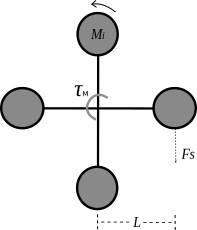
\includegraphics[width=6.5cm]{quadrotorTorque}    
		\caption{Motors torque experiment configuration} 
		\label{fig:quadrotortorque}
	\end{center}
\end{figure}
Taking into account that when the motor rotates clockwise, the quadrotor will tend to rotate counter-clockwise and vice versa, a scale is located to indirectly obtain the generated force $F_{s}$, using the reading of the weight $m_s$ as $F_{s} = m_{s}|\vec{g}|\ [N]$. Using (\ref{eqn:thrustvspwm}) and the \textit{PWM} width steps used in the motors thrust experiment, multiple $F_{M_i}$-dependent $F_s$ readings are obtained. The torques $\tau_M$ are then calculated by
\begin{equation}
\tau_{M} = F_{s}L\ [N\cdot m],
\end{equation}
and their results are shown in Fig. \ref{fig:torque_id}.
\begin{figure}[H]
	\begin{center}
		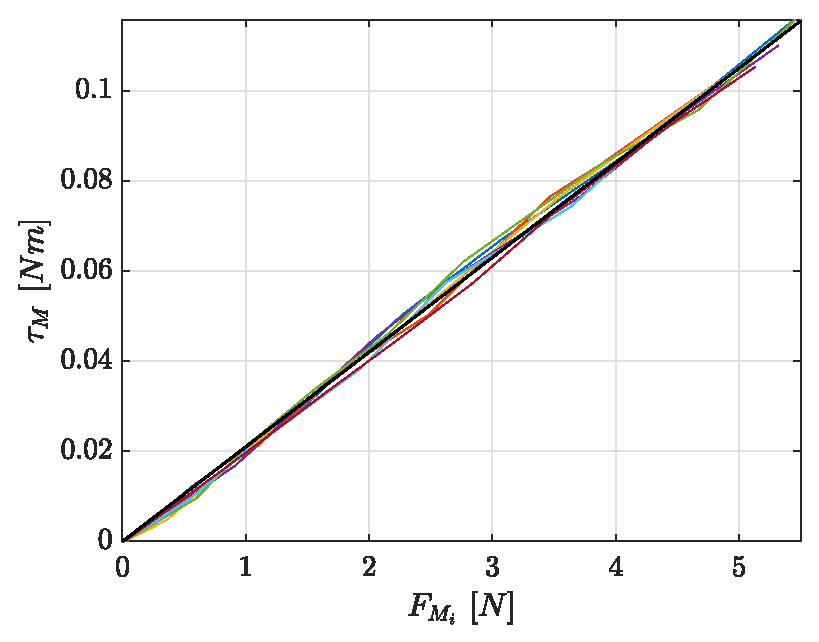
\includegraphics[width=9.5cm]{torque_id}    
		\caption{Torque} 
		\label{fig:torque_id}
	\end{center}
\end{figure}
The relation between $\tau_M$ and $F_{M_i}$ is linear as expected, and its slope defines the variable $K_m$ as
\begin{equation}
K_{m} = 0.021\ [m].
\end{equation}

\section{Conclusions}
This chapter presented the physical composition and parametrization of the smart- phone-based quadrotor prototype. In the first part, all the components of the quadrotor are detailed. A medium-size carbon fiber frame is used to support the complete quadrotor system. The LG Nexus 5X is selected as the smartphone where the control and estimation algorithms will be executed, which sends the control signals to an Arduino Mega ADK in order to generate \textit{PWM} signals that set the motors rotational velocities through the ESC. These components are supported and protected by 3D-printed objects that are attached to the carbon fiber frame. On the other hand, the system is parameterized in its entirety using experimental methods. Here, the total mass and moments of inertia of the system are defined using a scale and the bifilar pendulum experiment respectively, while the motor's thrust and torque about the $z$-axis are found applying multiple \textit{PWM} signals to the ESCs and obtaining the corresponding variable with the help of the scale.